\documentclass[../main.tex]{subfiles}

\begin{document}

In Chapter \ref{chap:implementation} we described that we can leverage the increased performance of the alignment algorithm to improve its accuracy by consenting the outputs of multiple runs. In this section we would like to analyze the results of this technique. To do so, we have tried repeating the alignment multiple times with slightly different galleries. We expect that good particles produce nearby results consistently, whilst bad particles produce random alignment parameters. Consequently as the number of repetitions increases, the confidence level of the alignment result also increases. The philosophy behind the consensus is that we prefer to use a few images that we have complete confidence in, rather than numerous images that lack our trust.

Regarding the particles that pass this consensus, the drop rate is not very large, meaning that most alignment results are consistent. The only exception to this rule is the EMPIAR-10256 dataset, which only preserves around $60 \si{\percent}$ of images after consensus. This is an expected result, as views separated by $90 \si{\degree}$ around the symmetry axis tend to be very similar. Thus, at this resolution-limit, assignments are practically random, leading to a lack of consensus. Preserved particles are either top views, side views with clear differences or side views where all assignments coincided by chance.

\begin{figure}[htbp]
    \centering
    \begin{subfigure}[b]{.8\textwidth}
         \centering
         \includegraphics[width=\linewidth]{results/consensus/simulated/kept}
         \caption{Simulated images}
    \end{subfigure}\\
    \vspace{2em}
    \begin{subfigure}[b]{.8\textwidth}
         \centering
         \includegraphics[width=\linewidth]{results/consensus/experimental/kept}
         \caption{Experimental images}
    \end{subfigure}
    \caption{Particle dropout ratio for different alignment repetitions}
    \label{fig:5:consensus_particles}
\end{figure}

As shown in Figures \ref{fig:5:consensus_angle_accuracy} and \ref{fig:5:consensus_shift_accuracy}, this consensus has a measurable positive outcome on the accuracy of the angle and shift assignments. The most significant improvement is obtained when only 3 repetitions are performed. Further repetitions still help to improve on the results, but accuracy increases are not as significant. Consequently, this technique helps to raise awareness of potential misalignment issues and enhances confidence in the obtained result.

\begin{figure}[htbp]
    \centering
    \begin{subfigure}[b]{.8\textwidth}
         \centering
         \includegraphics[width=\linewidth]{results/consensus/simulated/angle error}
         \caption{Simulated images}
    \end{subfigure}\\
    \vspace{2em}
    \begin{subfigure}[b]{.8\textwidth}
         \centering
         \includegraphics[width=\linewidth]{results/consensus/experimental/angle error}
         \caption{Experimental images}
    \end{subfigure}
    \caption{Angle accuracy for different alignment repetitions}
    \label{fig:5:consensus_angle_accuracy}
\end{figure}

\begin{figure}[htbp]
    \centering
    \begin{subfigure}[b]{.8\textwidth}
         \centering
         \includegraphics[width=\linewidth]{results/consensus/simulated/shift error}
         \caption{Simulated images}
    \end{subfigure}\\
    \vspace{2em}
    \begin{subfigure}[b]{.8\textwidth}
         \centering
         \includegraphics[width=\linewidth]{results/consensus/experimental/shift error}
         \caption{Experimental images}
    \end{subfigure}
    \caption{Shift accuracy for different alignment repetitions}
    \label{fig:5:consensus_shift_accuracy}
\end{figure}

This increased accuracy in alignment results do not always imply an improvement of the reconstruction resolution. Indeed, Figure \ref{fig:5:consensus_resolution} shows that in some cases this reduction in the number of particles has a negative effect on the resolution. As described earlier, the alignment errors do not have to be correlated with reconstruction errors, as more often than not, there are many highly compatible views, specially at low resolution. Thus, if a particle ``jumps'' across several compatible views, we decide that its pose is not conclusive; in spite of the map resolution increase that would involve using it.

\begin{figure}[htbp]
    \centering
    \begin{subfigure}[b]{.8\textwidth}
         \centering
         \includegraphics[width=\linewidth]{results/consensus/simulated/resolution}
         \caption{Simulated images}
    \end{subfigure}\\
    \vspace{2em}
    \begin{subfigure}[b]{.8\textwidth}
         \centering
         \includegraphics[width=\linewidth]{results/consensus/experimental/resolution}
         \caption{Experimental images}
    \end{subfigure}
    \caption{Reconstruction resolution for different alignment repetitions}
    \label{fig:5:consensus_resolution}
\end{figure}

Even though the angular consensus does not consistently help to increase the resolution of the reconstructed volume, it provides truthful alignment information to the posterior local alignment. These local alignments are heavily biased by the prior information. Thus, the starting point conditions the capability of local searches to find a global minima. Therefore, providing them with a reliable initial solution increases the odds of it reaching a local minima or at least reaching a deeper minima. This in turn will help to produce a final volume with a higher resolution.

\end{document}
